\documentclass[border=10pt]{standalone}
\usepackage[svgnames]{xcolor}
\usepackage{amsmath}
\usepackage{pgfplots}
\pgfplotsset{compat=newest}
\usepackage[sfdefault]{FiraSans}
\usepackage{FiraMono}
\renewcommand*\familydefault{\sfdefault}
\begin{document}
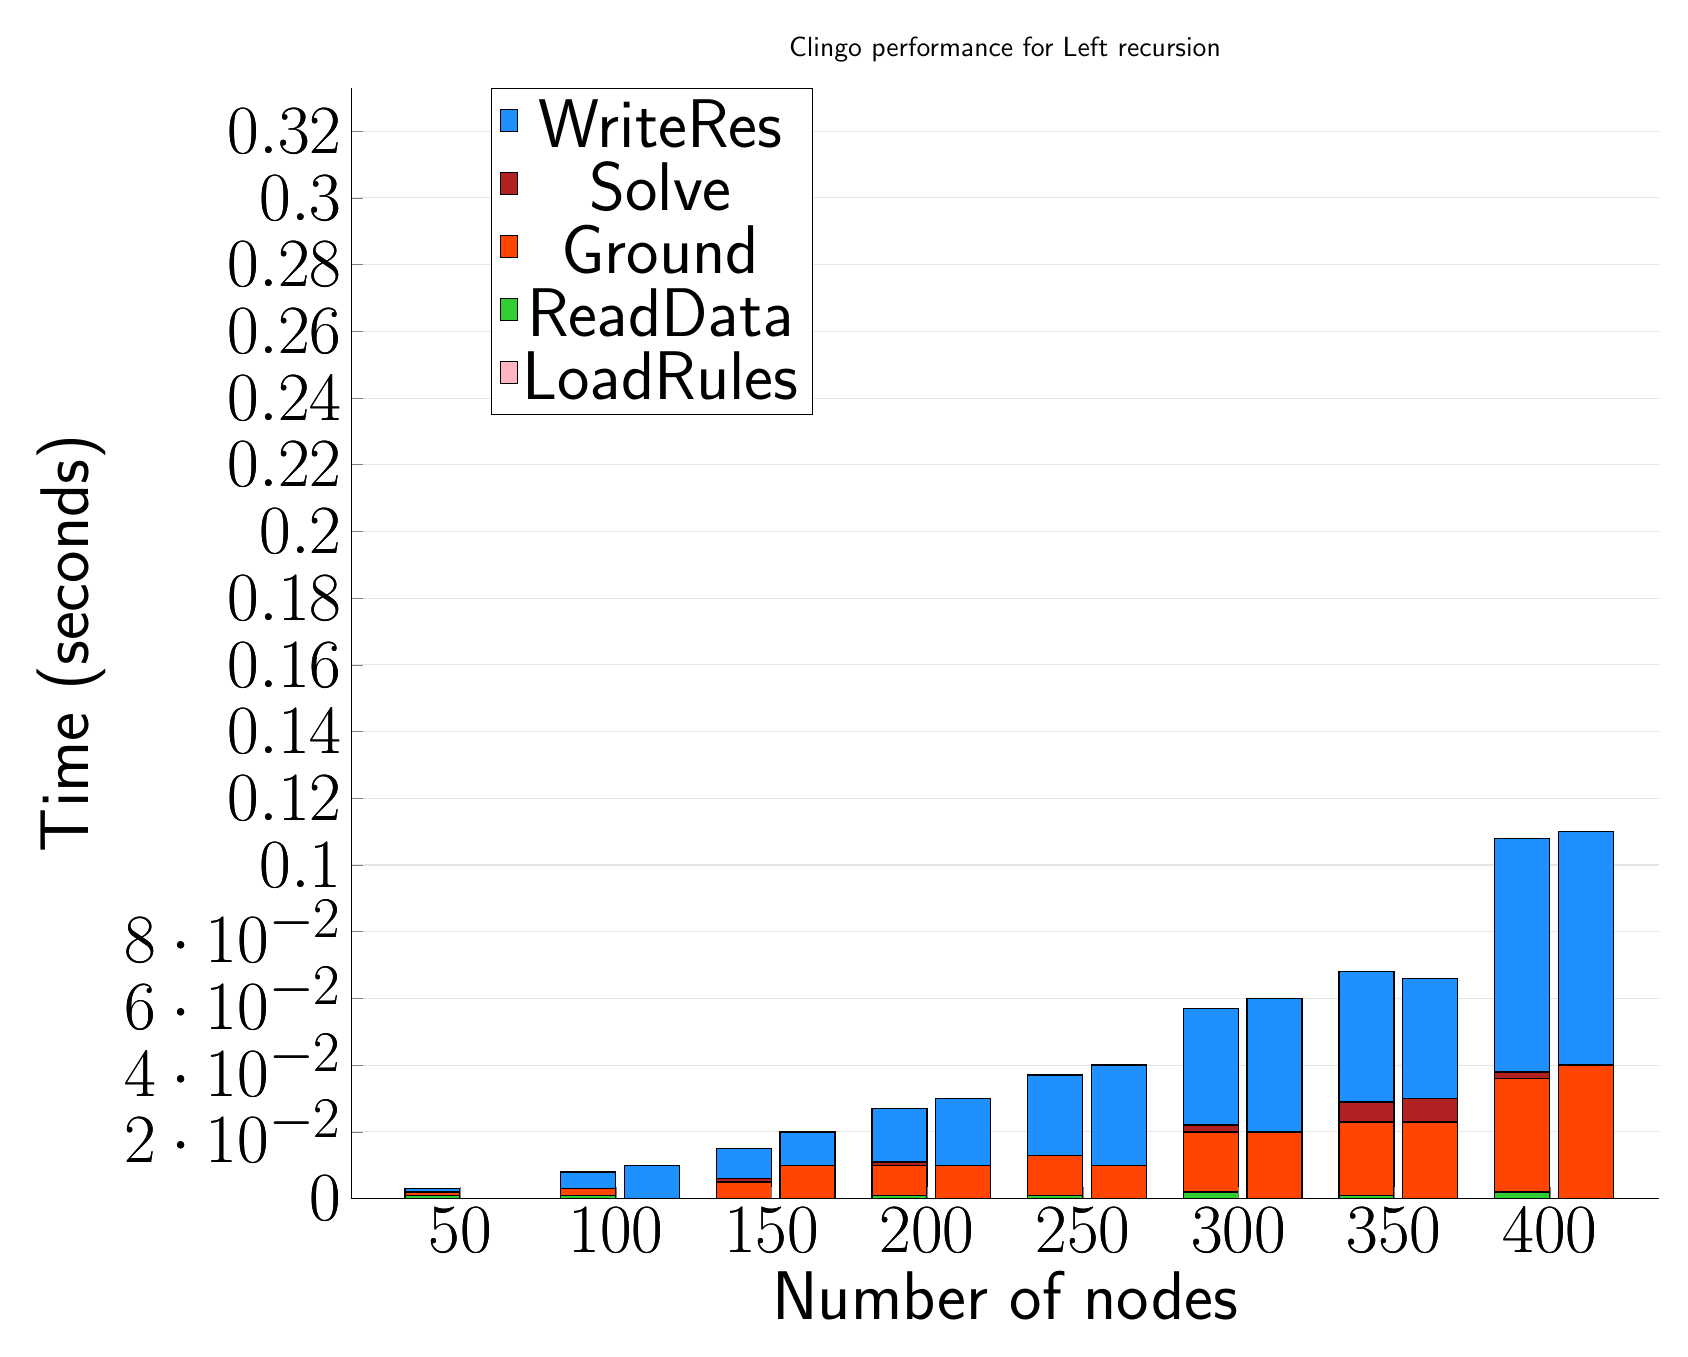
\begin{tikzpicture}
	\begin{axis}[
			ybar stacked,
			title={Clingo performance for Left recursion},
			bar shift=-10pt,
			width=1.5\textwidth,
			bar width=0.7cm,
			ymajorgrids, tick align=inside,
			major grid style={draw=gray!20},
			xtick=data,
			ymin=0, ymax=0.3330000114440918,
			axis x line*=bottom,
			axis y line*=left,
			enlarge x limits=0.1,
			legend style={
					at={(0.23, 1)},
					anchor=north,
					legend columns=1,
					font=\Huge,
				},
			ylabel={Time (seconds)},
			xlabel={Number of nodes},
			label style={font=\Huge},
			tick label style={font=\Huge},
		]
		\addlegendimage{fill=DodgerBlue, draw=black, line width=0.2pt}
		\addlegendentry{WriteRes}
		\addlegendimage{fill=FireBrick, draw=black, line width=0.2pt}
		\addlegendentry{Solve}
		\addlegendimage{fill=OrangeRed, draw=black, line width=0.2pt}
		\addlegendentry{Ground}
		\addlegendimage{fill=LimeGreen, draw=black, line width=0.2pt}
		\addlegendentry{ReadData}
		\addlegendimage{fill=LightPink, draw=black, line width=0.2pt}
		\addlegendentry{LoadRules}
		\addplot +[fill=LightPink, draw=black, line width=0.5pt] coordinates {
				(50, 0.0)
				(100, 0.0)
				(150, 0.0)
				(200, 0.0)
				(250, 0.0)
				(300, 0.0)
				(350, 0.0)
				(400, 0.0)
			};
		\addplot +[fill=LimeGreen, draw=black, line width=0.5pt] coordinates {
				(50, 0.0009999990463256836)
				(100, 0.0009999990463256836)
				(150, 0.0)
				(200, 0.0009999990463256836)
				(250, 0.0009999990463256836)
				(300, 0.0019999980926513673)
				(350, 0.0009999990463256836)
				(400, 0.0019999980926513673)
			};
		\addplot +[fill=OrangeRed, draw=black, line width=0.5pt] coordinates {
				(50, 0.0009999990463256836)
				(100, 0.0019999980926513673)
				(150, 0.004999995231628418)
				(200, 0.009000015258789063)
				(250, 0.012000012397766113)
				(300, 0.018000006675720215)
				(350, 0.02200000286102295)
				(400, 0.03399999141693115)
			};
		\addplot +[fill=FireBrick, draw=black, line width=0.5pt] coordinates {
				(50, 0.0)
				(100, 0.0)
				(150, 0.0009999990463256836)
				(200, 0.0009999990463256836)
				(250, 0.0)
				(300, 0.0019999980926513673)
				(350, 0.005999994277954101)
				(400, 0.0019999980926513673)
			};
		\addplot +[fill=DodgerBlue, draw=black, line width=0.5pt] coordinates {
				(50, 0.0009999990463256836)
				(100, 0.005000019073486328)
				(150, 0.009000015258789063)
				(200, 0.016000008583068846)
				(250, 0.024000000953674317)
				(300, 0.03499999046325684)
				(350, 0.03899998664855957)
				(400, 0.0700000286102295)
			};
	\end{axis}
	\begin{axis}[
			ybar stacked,
			bar shift=13pt,
			width=1.5\textwidth,
			bar width=0.7cm,
			ymajorgrids, tick align=inside,
			major grid style={draw=none},
			xtick=data,
			ymin=0, ymax=0.3330000114440918,
			axis x line*=none,
			axis y line*=none,
			enlarge x limits=0.1,
			label style={font=\Huge},
			tick label style={font=\Huge},
		]
		\addplot +[fill=LightPink, draw=black, line width=0.5pt] coordinates {
				(50, 0.0)
				(100, 0.0)
				(150, 0.0)
				(200, 0.0)
				(250, 0.0)
				(300, 0.0)
				(350, 0.0)
				(400, 0.0)
			};
		\addplot +[fill=LimeGreen, draw=black, line width=0.5pt] coordinates {
				(50, 0.0)
				(100, 0.0)
				(150, 0.0)
				(200, 0.0)
				(250, 0.0)
				(300, 0.0)
				(350, 0.0)
				(400, 0.0)
			};
		\addplot +[fill=OrangeRed, draw=black, line width=0.5pt] coordinates {
				(50, 0.0)
				(100, 0.0)
				(150, 0.009999999999999997)
				(200, 0.009999999999999997)
				(250, 0.009999999999999997)
				(300, 0.019999999999999997)
				(350, 0.023)
				(400, 0.03999999999999999)
			};
		\addplot +[fill=FireBrick, draw=black, line width=0.5pt] coordinates {
				(50, 0.0)
				(100, 0.0)
				(150, 0.0)
				(200, 0.0)
				(250, 0.0)
				(300, 0.0)
				(350, 0.007000000000000001)
				(400, 0.0)
			};
		\addplot +[fill=DodgerBlue, draw=black, line width=0.5pt] coordinates {
				(50, 0.0)
				(100, 0.009999999999999997)
				(150, 0.010000000000000004)
				(200, 0.020000000000000007)
				(250, 0.030000000000000006)
				(300, 0.039999999999999994)
				(350, 0.03599999999999999)
				(400, 0.07000000000000002)
			};
	\end{axis}
\end{tikzpicture}

\end{document}
